
%(BEGIN_QUESTION)
% Copyright 2008, Tony R. Kuphaldt, released under the Creative Commons Attribution License (v 1.0)
% This means you may do almost anything with this work of mine, so long as you give me proper credit

Complete the table of values for this circuit.  Be sure to show all your work!

$$\includegraphics[width=15.5cm]{i03239x01.eps}$$

As you solve this problem, be sure to store all intermediate calculations (i.e. answers given to you by your calculator which you will use later in the problem) in your calculator's memory locations, so as to avoid re-entering those values by hand.  Re-entering calculated values unnecessarily introduces rounding errors into your work, as well as invites keystroke errors.  {\it Avoiding the unnecessary introduction of error is a very important concept in Instrumentation!}

If your final answers are rounded as a result of not doing this, you will only receive half-credit for your work.  This is a general policy for all your mathematical work in this program, not just this particular problem!


\vfil 

Note: the task of analyzing any series-parallel resistor network is greatly simplified by an approach outlined in the online textbook {\it Lessons In Electric Circuits}, in the ``Series-Parallel Combination Circuits'' chapter.  There, a technique is demonstrated by which one may reduce a complex series-parallel network step-by-step into a single equivalent resistance.  After this reduction, Ohm's Law and Kirchhoff's Laws of voltage and current are applied while ``expanding'' the circuit back into its original form.  Even though the current notation in this textbook is electron flow rather than conventional flow, the series-parallel analysis technique works all the same.

\underbar{file i03239}
\eject
%(END_QUESTION)





%(BEGIN_ANSWER)

This is a graded question -- no answers or hints given!

%(END_ANSWER)





%(BEGIN_NOTES)

$$\includegraphics[width=15.5cm]{i03239x02.eps}$$

%INDEX% Electronics review: series-parallel circuits

%(END_NOTES)

